\documentclass{beamer}
\mode <presentation>
{
    \usetheme{boxes}
    \usecolortheme{crane}
    \setbeamercovered{transparent}
}
\definecolor{craneorange}{RGB}{220,197, 90}

\usepackage{pgf,pgfarrows,pgfnodes}
\usepackage[english]{babel}
\usepackage{times}
\usepackage{amsmath}
% math extension - one probably wants to use symbols like '[' (written as '$[$')
\usepackage{ucs}
%\usepackage[utf8]{inputenc}
\usefonttheme{structuresmallcapsserif}

% utf8x does not work with xetex
\usepackage{ifxetex}
\ifxetex
\else
        \usepackage[utf8x]{inputenc}
\fi

\usepackage[normalem]{ulem}

%\setbeamercolor{background canvas}{bg=
\includegraphics[width=\textwidth]{./pics/wolf.png}}

\title{Assets management with GLPI}
\author{\href{http://www.FusionInventory.org}{FusionInventory.org}}
\subject{Assets management with FusionInventory and GLPI}
\keywords{Assets management, Inventory, FusionInventory, GLPI}

\date{LinuxTag 2011}
\titlegraphic{GLPI and FusionInventory}
%subtitle{
\includegraphics[width=1.2cm]{./pics/fusioninventory-logo.png}}
\institute{
\includegraphics[height=3.2cm]{./pics/logos/Logo_LinuxTag.pdf}}
\author{ Gonéri Le Bouder and Walid Nouh }
\logo{
\includegraphics[height=0.7cm]{./pics/logos/glpi+fusinv_small.jpg}}

\AtBeginSection[] % Do nothing for \section*
{
    \begin{frame}<beamer>
        \frametitle{Outline}
    \tableofcontents[currentsection]
        \end{frame}
}


%%%%%%%%%%%%%%%%%%%%%%%%%%%%%%%%%%%%%%%%%%%%%%%
%%%%%%%%%%%%%%%%%%%%%%%%%%%%%%%%%%%%%%%%%%%%%%%
\begin{document}

\frame[plain]{\titlepage}

\begin{frame}
    \frametitle{About us: Walid Nouh}
<<<<<<< HEAD
IT management consultant
    \begin{itemize}
    \item GLPI core developer
    \item FusionInventory project co-leader
    \item Quadskate fanatic
    \item Work at TECLIB', Brussels, Belgium
    \end{itemize}
=======

    \begin{block}{IT management consultant}
        \begin{itemize}
        \item GLPI core developer
        \item FusionInventory project co-leader
        \item Rollerskate fanatic
        \item Work at TECLIB', Brussels, Belgium
        \end{itemize}
    \end{block}
>>>>>>> c33110151a9501e3e4285e3f62e2cd3f61f6d30c

\end{frame}



\begin{frame}
    \frametitle{About us: Gonéri Le Bouder}


    \begin{block}{Free software enthusiast}
        \begin{itemize}
        \item Debian Developer
        \item Perl Monger
        \item Former OCS Inventory developer
        \item FusionInventory project co-leader
        \item Work at TECLIB', Paris, France
        \item {\tiny and an awful french accent}
        \end{itemize}
    \end{block}

\end{frame}


\section{What is GLPI for?}


\begin{frame}
    \frametitle{What is GLPI for?}

 \begin{columns}
 \begin{column}{0.35\textwidth}
         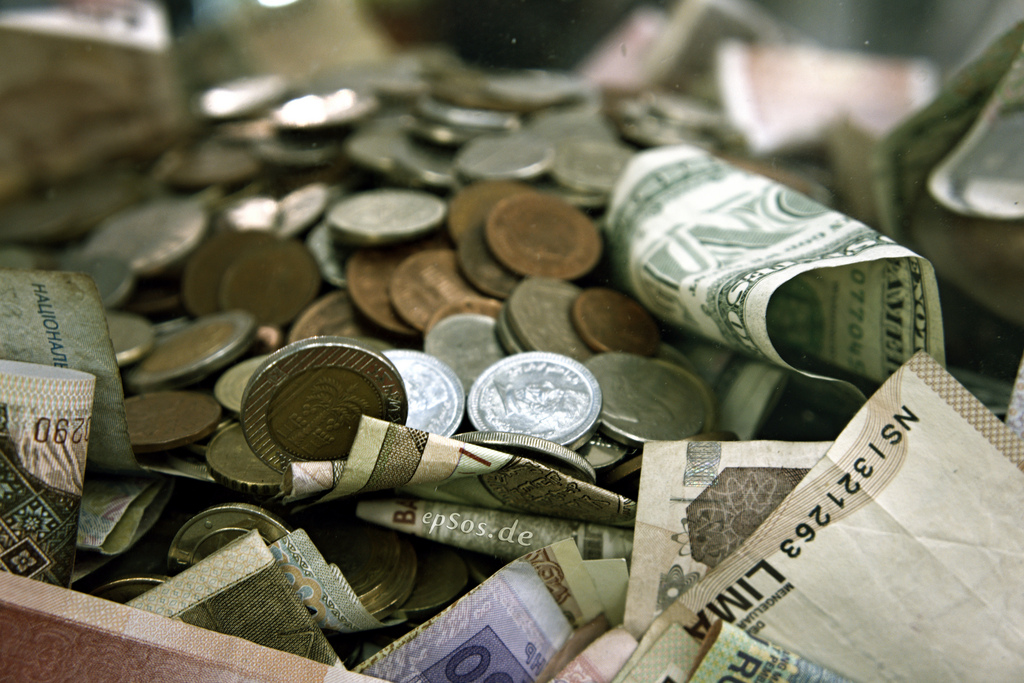
\includegraphics[height=7.5cm]{./pics/purchasing.jpg}
 \end{column}
 \begin{column}{0.65\textwidth}
    \begin{block}{The purchasing department}
        \begin{itemize}
            \item How much did we spend last year with IBM?
            \item Is the paternship with Oracle still running?
            \item How many and where are the assets bought with last year budget?
        \end{itemize}
    \end{block}
 \end{column}
\end{columns}



\end{frame}

\begin{frame}
    \frametitle{What is GLPI for?}

 \begin{columns}
 \begin{column}{0.35\textwidth}
         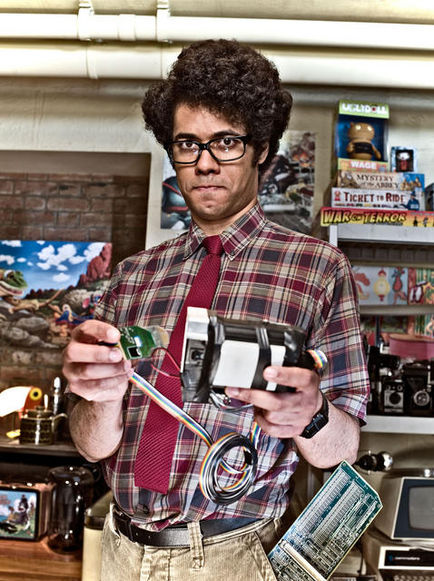
\includegraphics[height=7.5cm]{./pics/itcrowd.jpg}
 \end{column}
 \begin{column}{0.65\textwidth}
    \begin{block}{The IT crowd}
        \begin{itemize}
            \item How many server still run with 2GB of memory?
            \item Do we still have those old Toshiba laptop?
            \item Do our servers have the lastest security fixes?
        \end{itemize}
    \end{block}
 \end{column}
\end{columns}

 \end{frame}

\begin{frame}
    \frametitle{What is GLPI for?}

 \begin{columns}
 \begin{column}{0.1\textwidth}
         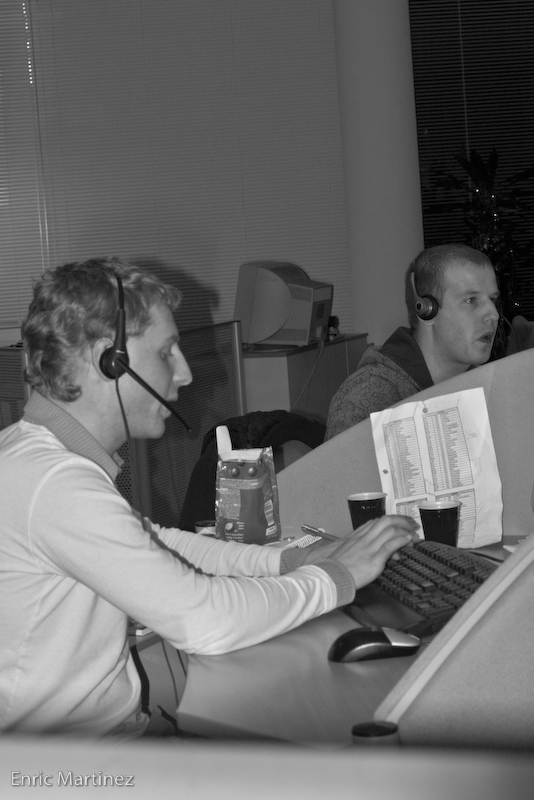
\includegraphics[height=7.5cm]{./pics/helpdesk.jpg}
 \end{column}
 \begin{column}{1\textwidth}

    \begin{block}{The Service Desk team}
        \begin{itemize}
            \item Mr Jones computer is out of order, what happend?
            \item Oh the printer ink cartridge is running \\
                low on the second floor!
        \end{itemize}
    \end{block}
 \end{column}
\end{columns}


\end{frame}

\begin{frame}
    \frametitle{What is GLPI for?}

 \begin{columns}
 \begin{column}{0.35\textwidth}
         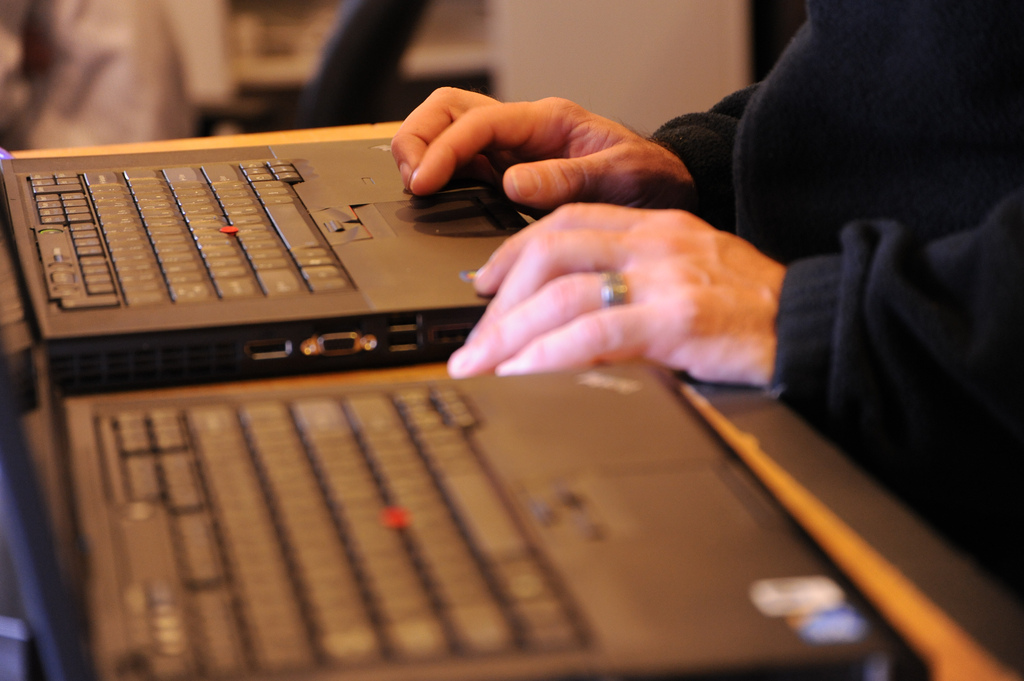
\includegraphics[height=7.5cm]{./pics/lenovo.jpg}
 \end{column}
 \begin{column}{0.65\textwidth}

    \begin{block}{The users}
        \begin{itemize}
            \item Why I can't print?
            \item Why I can't send email anymore?
            \item Are the IT guys really working on my request?
        \end{itemize}
    \end{block}
 \end{column}
\end{columns}

\end{frame}

\begin{frame}
    \frametitle{What is GLPI for?}

 \begin{columns}
 \begin{column}{0.15\textwidth}
         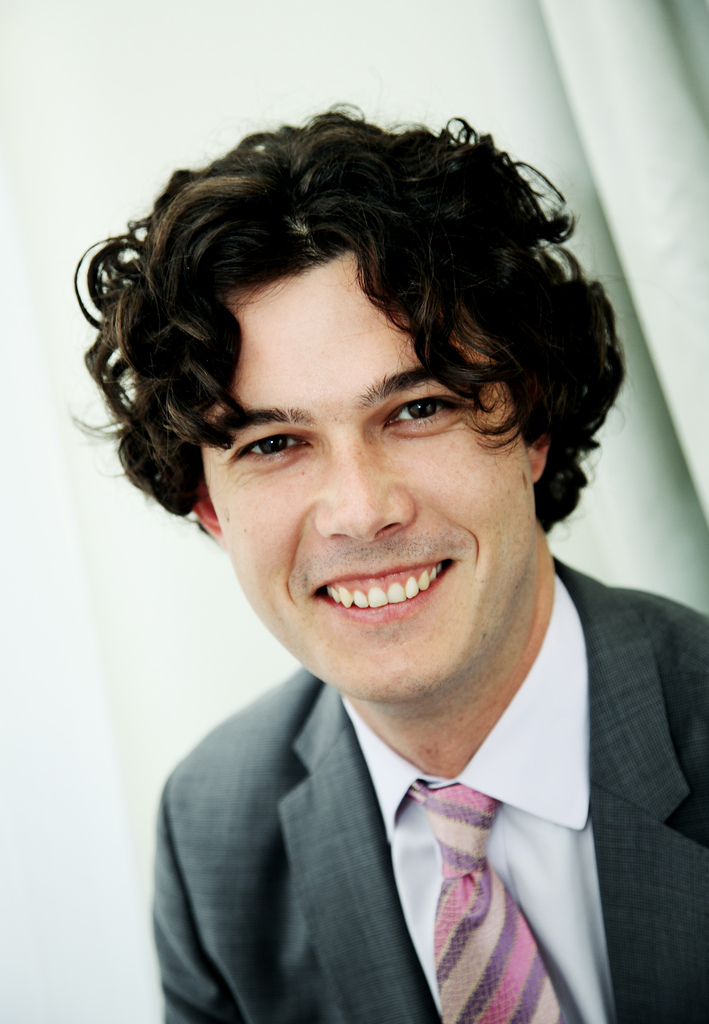
\includegraphics[height=8.5cm]{./pics/manager.jpg}
 \end{column}
 \begin{column}{1.25\textwidth}
    \begin{block}{The management}
        \begin{itemize}
            \item How many request per day get the support team?
            \item What is the user satisfaction level?
            \item I need more dashboards!
        \end{itemize}
    \end{block}
 \end{column}
\end{columns}


\end{frame}




\begin{frame}
    \frametitle{Installation 1/3}

         \pgfputat{\pgfxy(-1,-3)}{\pgfbox[left,top]{
\includegraphics[height=2.5cm]{./pics/php-mysql.jpg}}}
    \begin{block}{Easy step}
        \begin{itemize}
            \item Common web application
            \item Very few OS dependency
        \end{itemize}
    \end{block}

    Extract, run the wizard, your done!





\end{frame}

\begin{frame}
    \frametitle{Installation 2/3}


 \begin{columns}
 \begin{column}{0.34\textwidth}
    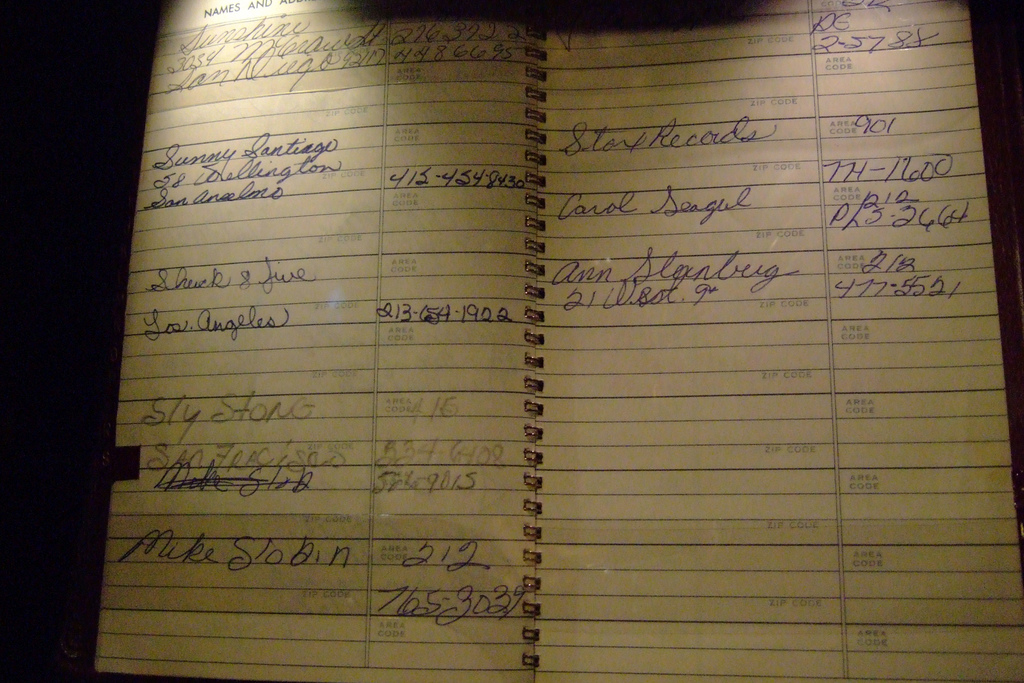
\includegraphics[height=6.5cm]{pics/addressbook.jpg}
 \end{column}
 \begin{column}{0.90\textwidth}
    \begin{block}{Easy, really? I want LDAP support! Ahah}
        \begin{itemize}
            \item Strong LDAP integration
            \item LDAP v3 compatible \\
            {\small ActiveDirectory, OpenLDAP, ...}
        \end{itemize}
    \end{block}

    \begin{block}{And more}
        \begin{itemize}
            \item POP3
            \item IMAP
        \end{itemize}
    \end{block}
 \end{column}
\end{columns}
\end{frame}

\begin{frame}
    \frametitle{Installation 3/3}


 \begin{columns}
 \begin{column}{0.34\textwidth}
    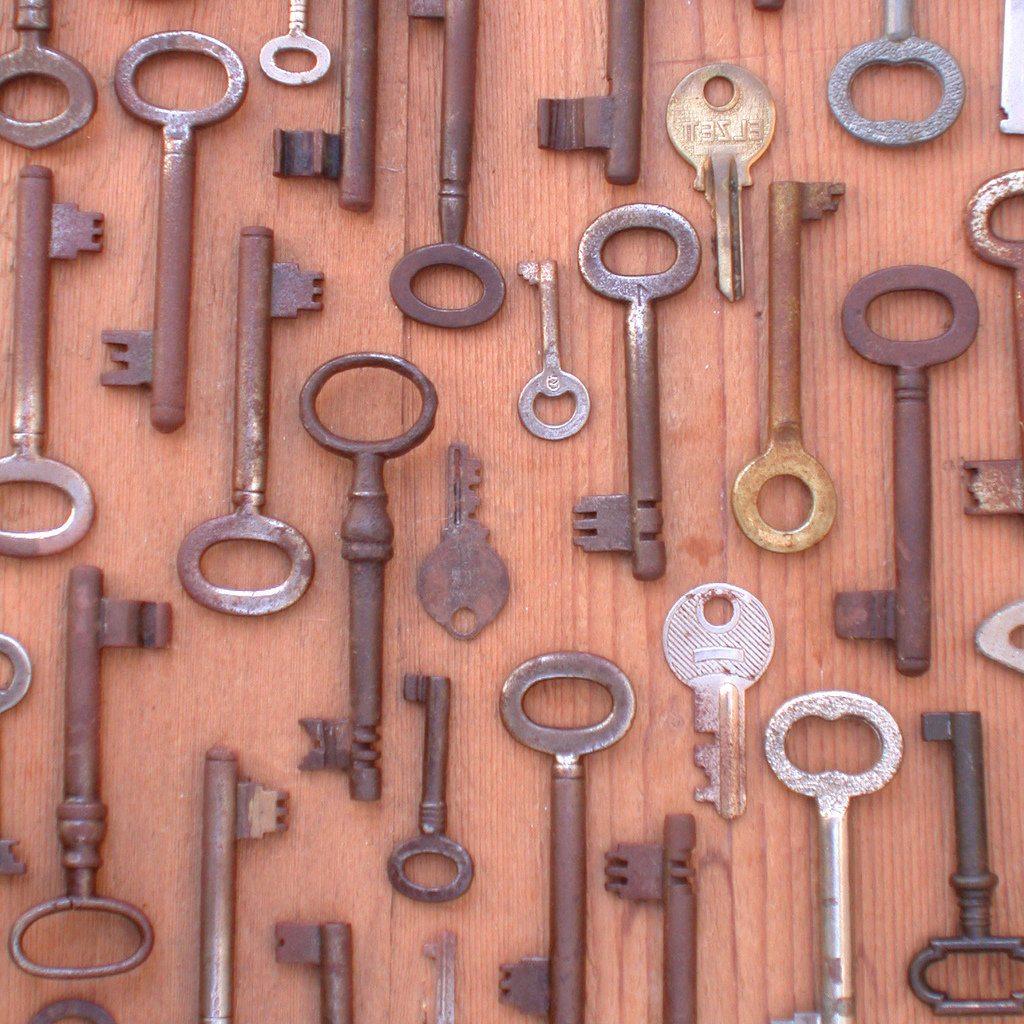
\includegraphics[height=10.5cm]{pics/sso.jpg}
 \end{column}
 \begin{column}{0.90\textwidth}
    \begin{block}{That was trivial, but I want SSO too!}
        \begin{itemize}
            \item WebSSO
            \item CAS
        \end{itemize}
    \end{block}
 \end{column}
\end{columns}

\end{frame}

\begin{frame}
    \frametitle{Architecture}

 \begin{columns}
 \begin{column}{0.34\textwidth}
 \end{column}
 \begin{column}{0.90\textwidth}
    
\includegraphics[height=6.5cm]{pics/scale.pdf}
 \end{column}
\end{columns}

\end{frame}

\begin{frame}
    \frametitle{Architecture}

 \begin{columns}
 \begin{column}{0.34\textwidth}
    \begin{block}{Really?}
        \begin{itemize}
            \item Existing large installation of GLPI \\
            {\small up to 130K computer inventoried}
            \item 1 million computer referenced so far and still growing
        \end{itemize}
    \end{block}

 \end{column}
 \begin{column}{0.90\textwidth}
    
\includegraphics[height=6.5cm]{pics/scale.pdf}

 \end{column}
\end{columns}

\end{frame}


\section{Collect your information}

\begin{frame}
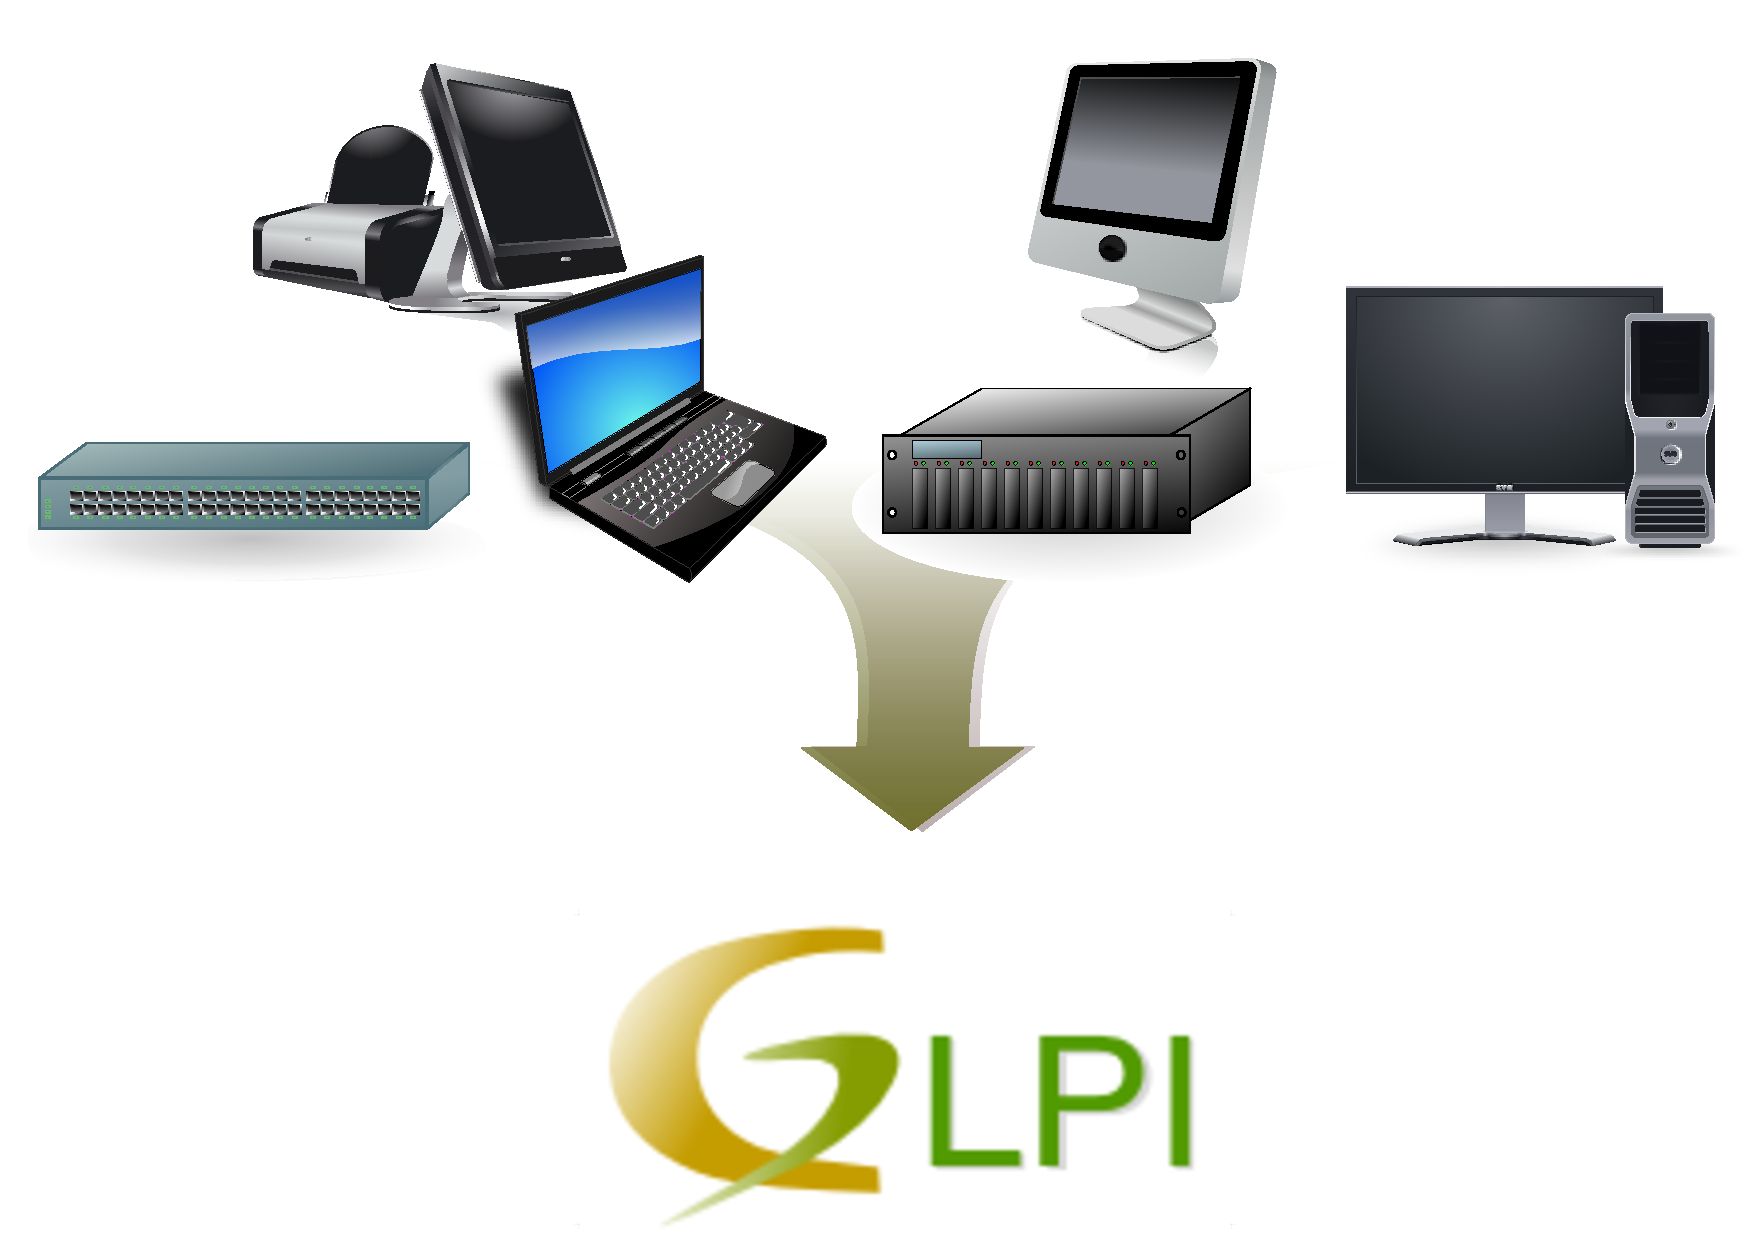
\includegraphics[height=6.5cm]{pics/bigpicture.pdf}
\end{frame}


\begin{frame}

    \frametitle{Collect your information}

 \begin{columns}
 \begin{column}{0.34\textwidth}
    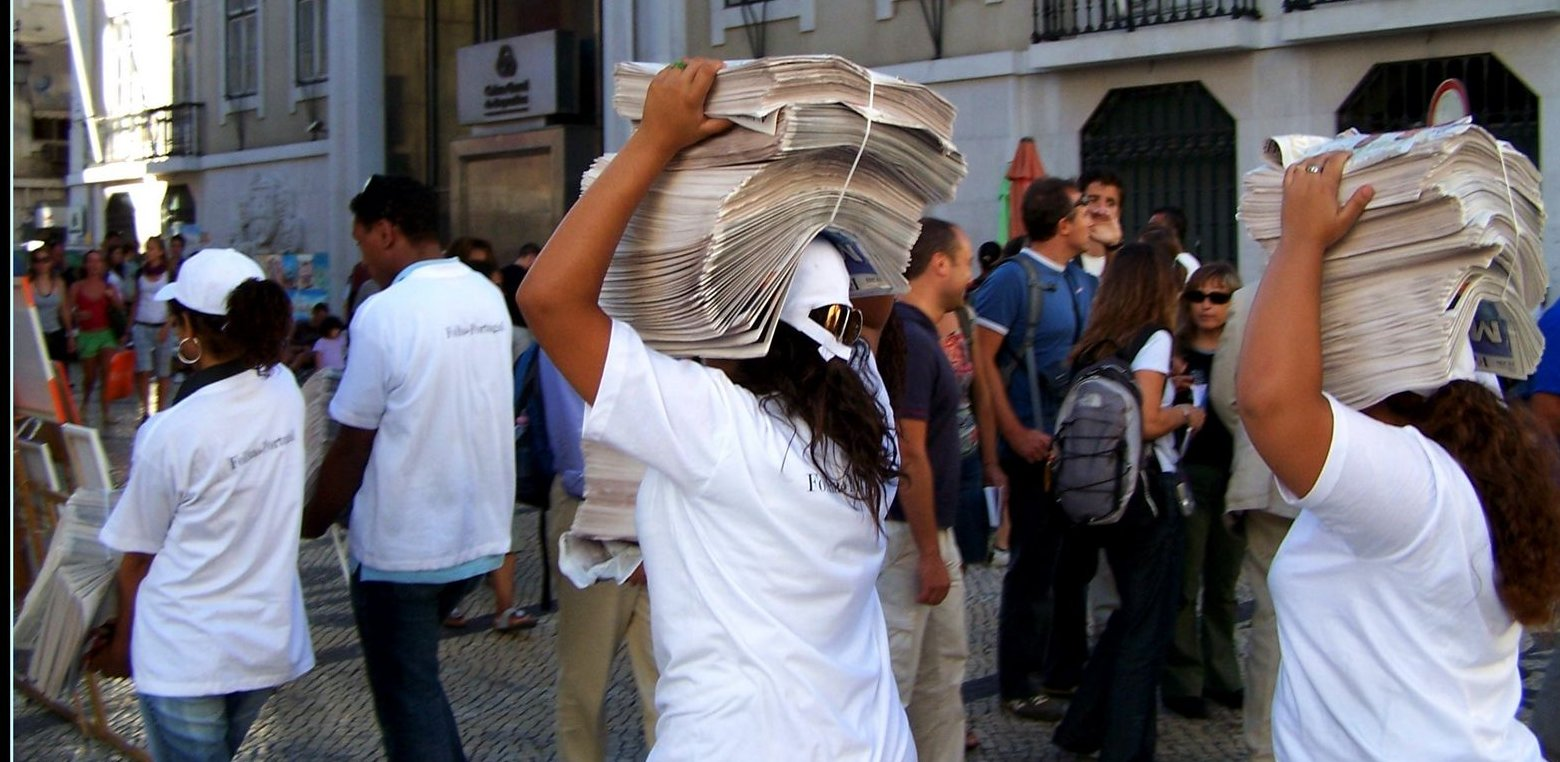
\includegraphics[height=6.5cm]{pics/information.jpg}
 \end{column}
 \begin{column}{0.90\textwidth}
 \end{column}
\end{columns}


\end{frame}



\begin{frame}

    \frametitle{Collect your information}

 \begin{columns}
 \begin{column}{0.34\textwidth}
    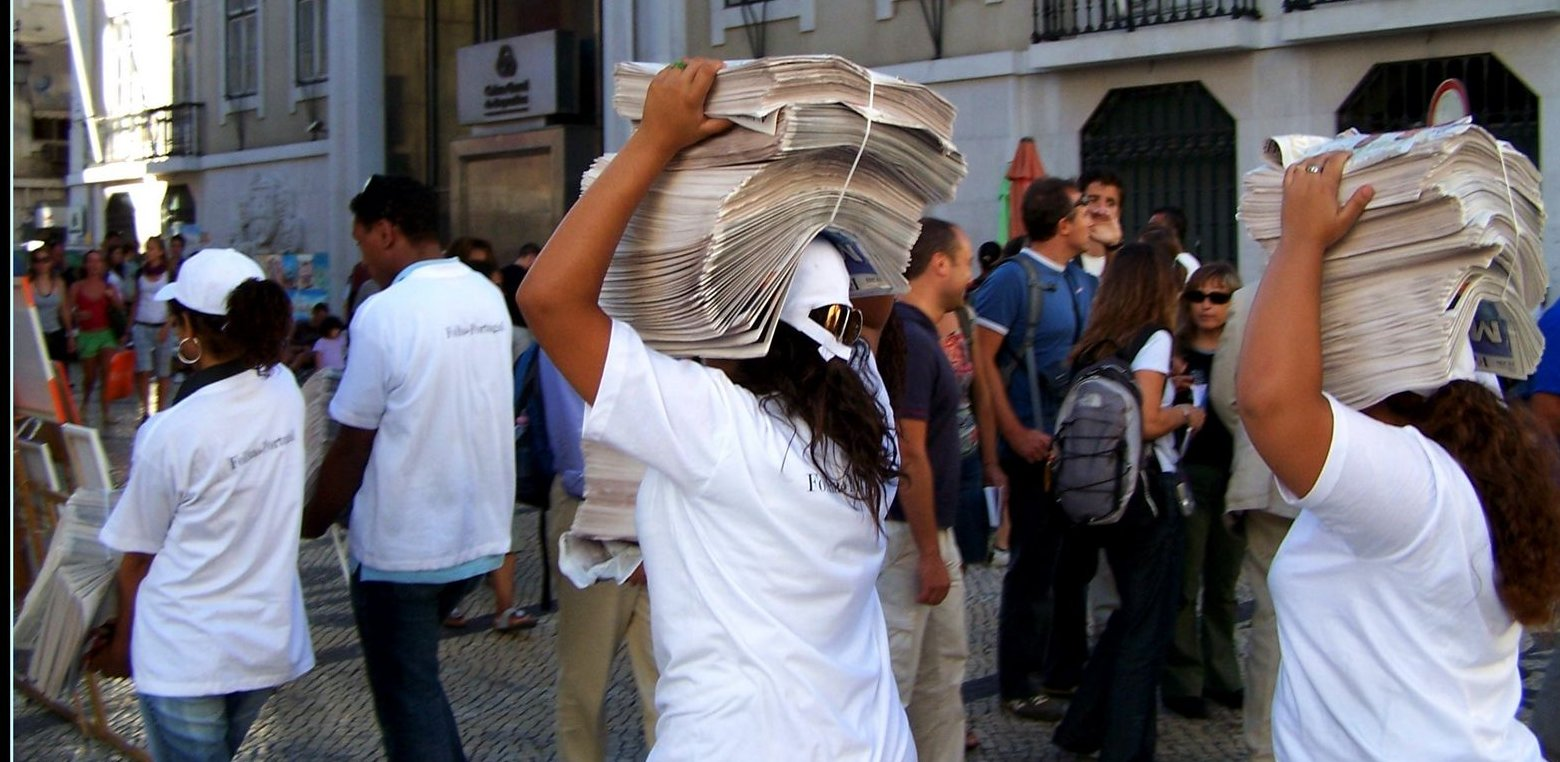
\includegraphics[height=6.5cm]{pics/information.jpg}
 \end{column}
 \begin{column}{0.90\textwidth}
    \begin{block}{Inputs}
        \begin{itemize}
            \item desktop computers and server
            \item network devices
            \item data coming from legacy system
            \item financial information
            \item ...
        \end{itemize}
    \end{block}

 \end{column}
\end{columns}


\end{frame}

\begin{frame}

    \frametitle{Computer}
 \begin{columns}
 \begin{column}{0.15\textwidth}
         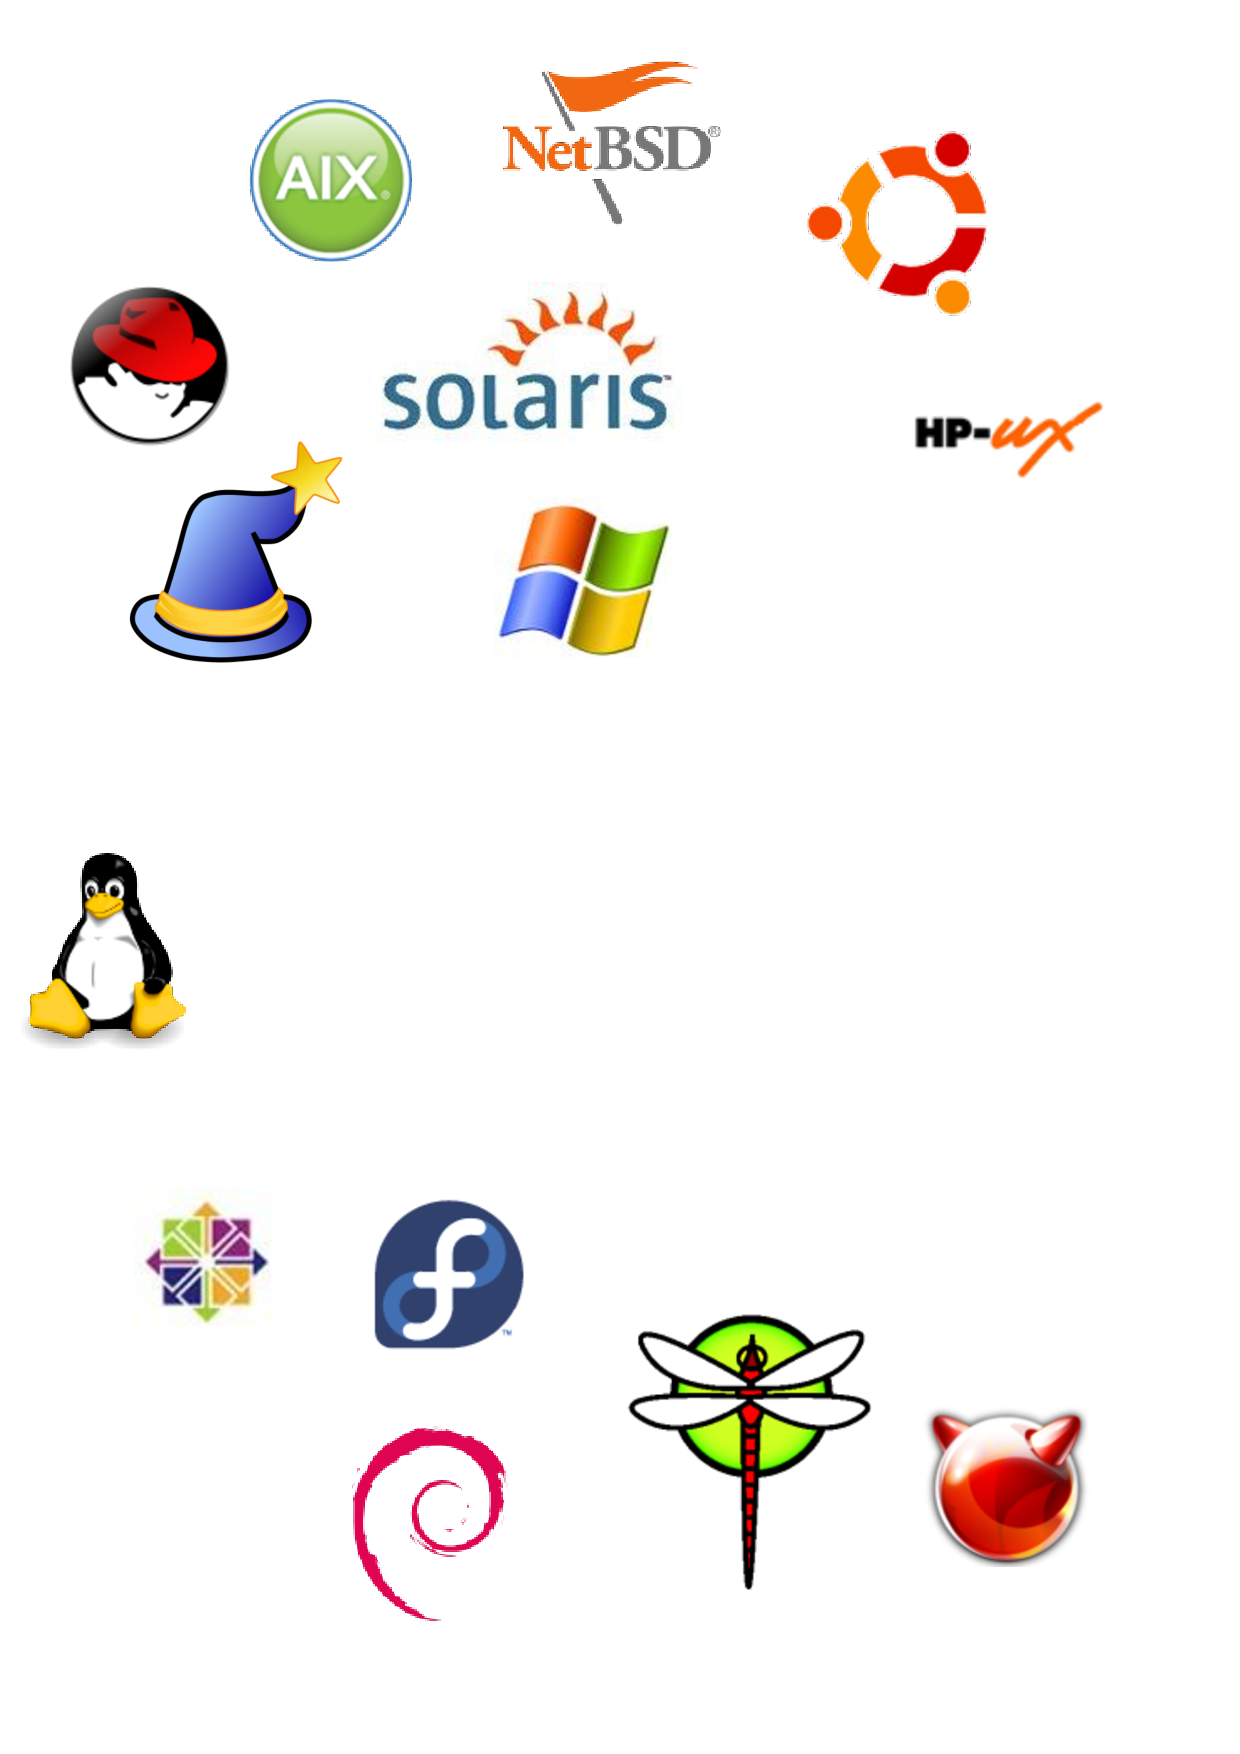
\includegraphics[height=8.5cm]{./pics/os.pdf}
 \end{column}
 \begin{column}{1.25\textwidth}
    \begin{block}{Easy step}
        \begin{itemize}
            \item Agent packaged for most of the OS
            \item Ready to use, no build, no dependency!
        \end{itemize}
    \end{block}


 \end{column}
\end{columns}




\end{frame}

\begin{frame}

    \frametitle{Network devices}


 \begin{columns}
 \begin{column}{0.15\textwidth}
         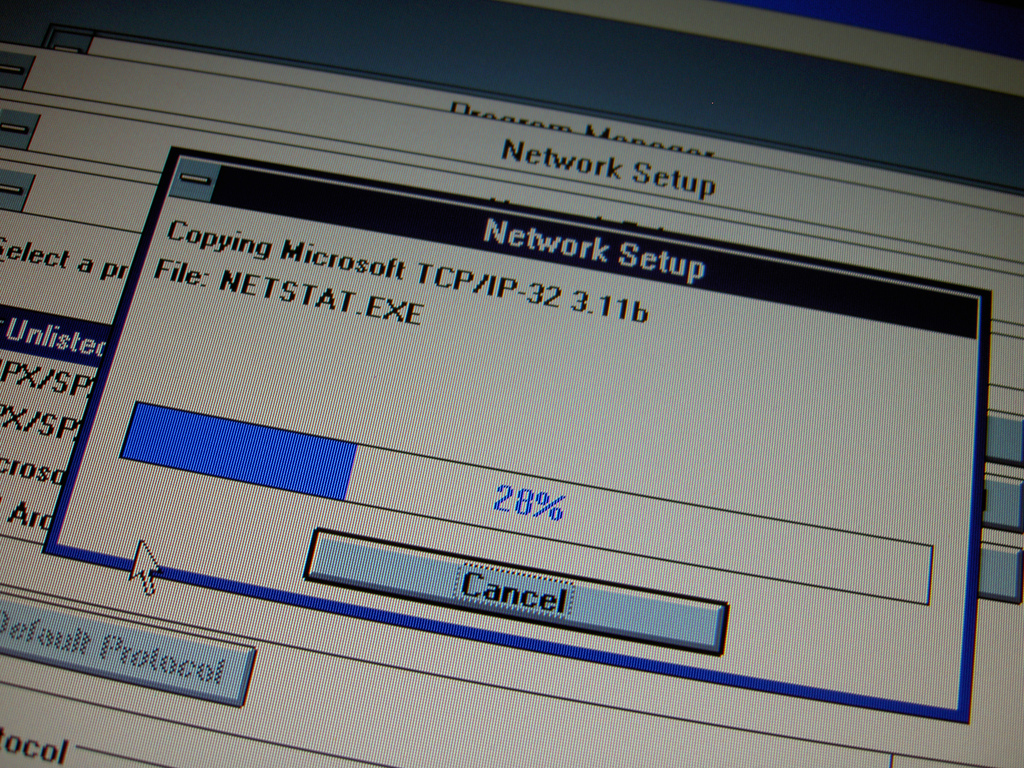
\includegraphics[height=8.5cm]{./pics/networking.jpg}
 \end{column}
 \begin{column}{1.25\textwidth}
    

    \begin{block}{routers, switchs, printers, wifi AP, etc \\
    FusionInventory do it remotely for you}
        \begin{itemize}
            \item Nothing to install
            \item Network scan to identify asset
            \item Use SNMP to collect information
        \end{itemize}
    \end{block}

 \end{column}
\end{columns}
\end{frame}


\begin{frame}

    \frametitle{Network devices}


 \begin{columns}
 \begin{column}{0.15\textwidth}
         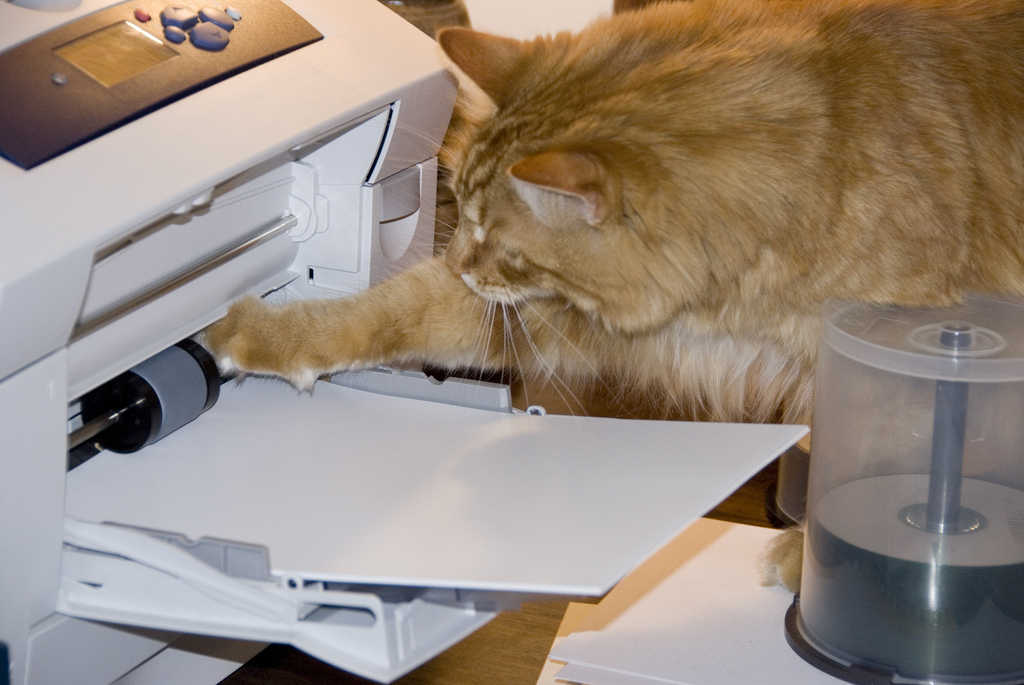
\includegraphics[height=8.5cm]{./pics/printer.jpg}
 \end{column}
 \begin{column}{1.25\textwidth}
    

    \begin{block}{routers}
        \begin{itemize}
            \item Cartridge ink levels
            \item Counter and statistics
        \end{itemize}
    \end{block}

 \end{column}
\end{columns}
\end{frame}



\begin{frame}




    \frametitle{Existing Inventory system}

 
    \begin{block}{What about my current system?}
        \begin{itemize}
            \item Financial information
            \item License
            \item Helpdesk
        \end{itemize}
    \end{block}
   

\end{frame}

\begin{frame}

    \frametitle{Application integration}
 \begin{columns}
 \begin{column}{0.45\textwidth}
         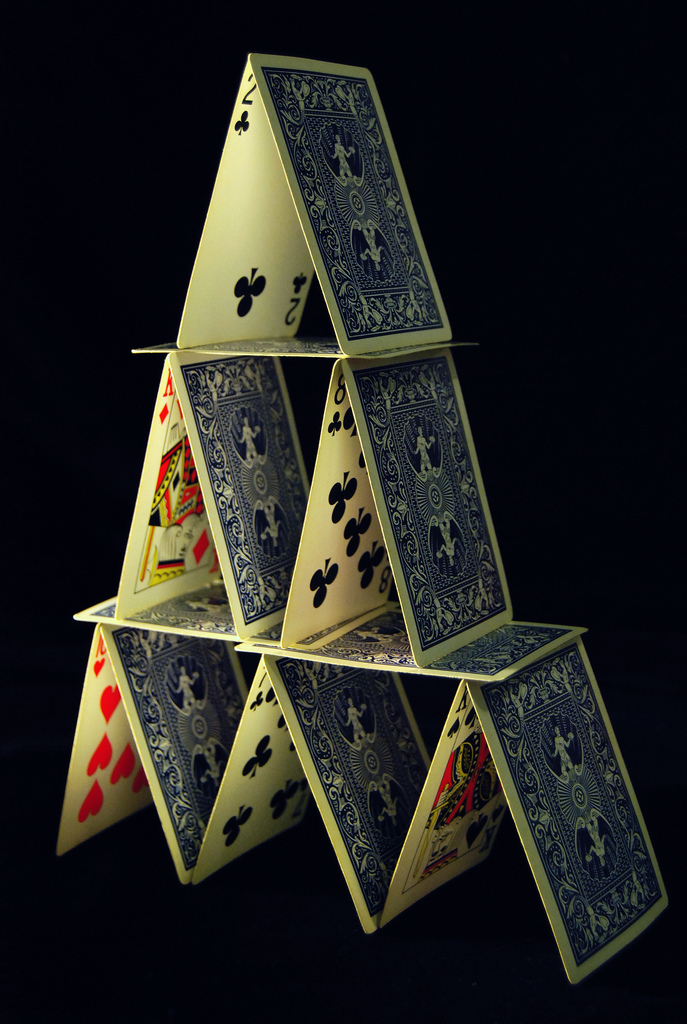
\includegraphics[height=7.5cm]{./pics/house_of_cards.jpg}
 \end{column}
 \begin{column}{0.45\textwidth}
     \begin{block}{Wait, some tools are already running here! \\
     How to interacte with them?}
        \begin{itemize}
            \item webservice interface
            \item plugin API
            \item CSV import/export
            \item ETL
        \end{itemize}
    \end{block}
   
 \end{column}
\end{columns}
\end{frame}


\begin{frame}

    \frametitle{Application integration: plugin}

    \begin{block}{A large collection of extension}
        \begin{itemize}
            \item Add load of new features
            \item Great integration in GLPI
        \end{itemize}
    \end{block}

\end{frame}




\section{Service Desk}

\begin{frame}

    \frametitle{Service Desk: the big picture}

    \begin{block}{ITIL v1 including}
        \begin{itemize}
            \item Incident management
            \item Business rules
            \item Notifications, multilingual support
        \end{itemize}
    \end{block}


\end{frame}

\begin{frame}

    \frametitle{Service Desk: the interfaces 1/2}

    \begin{block}{Web interfaces}
        \begin{itemize}
            \item End user simplified interface
            \item IT and technician standard interface
            \item Smartphones interface
        \end{itemize}
    \end{block}

\end{frame}
\begin{frame}

    \frametitle{Service Desk: the interfaces 2/2}

    \begin{block}{Webservice}
        \begin{itemize}
            \item to integrate GLPI in another system
            \item to push tickets into another helpdesk software
            \item or the opposite
        \end{itemize}
    \end{block}

    \begin{block}{Mail}
       \begin{itemize}
            \item send notification
            \item add and update tickets
       \end{itemize}
    \end{block}


\end{frame}

\section{Reporting}

\begin{frame}

    \frametitle{Service Desk: the big picture}

    \begin{block}{ITIL v1 including}
        \begin{itemize}
            \item Incident management
            \item Business rules
            \item Notifications, multilingual support
        \end{itemize}
    \end{block}


\end{frame}



\section{What else}

\begin{frame}

    \frametitle{What Else}


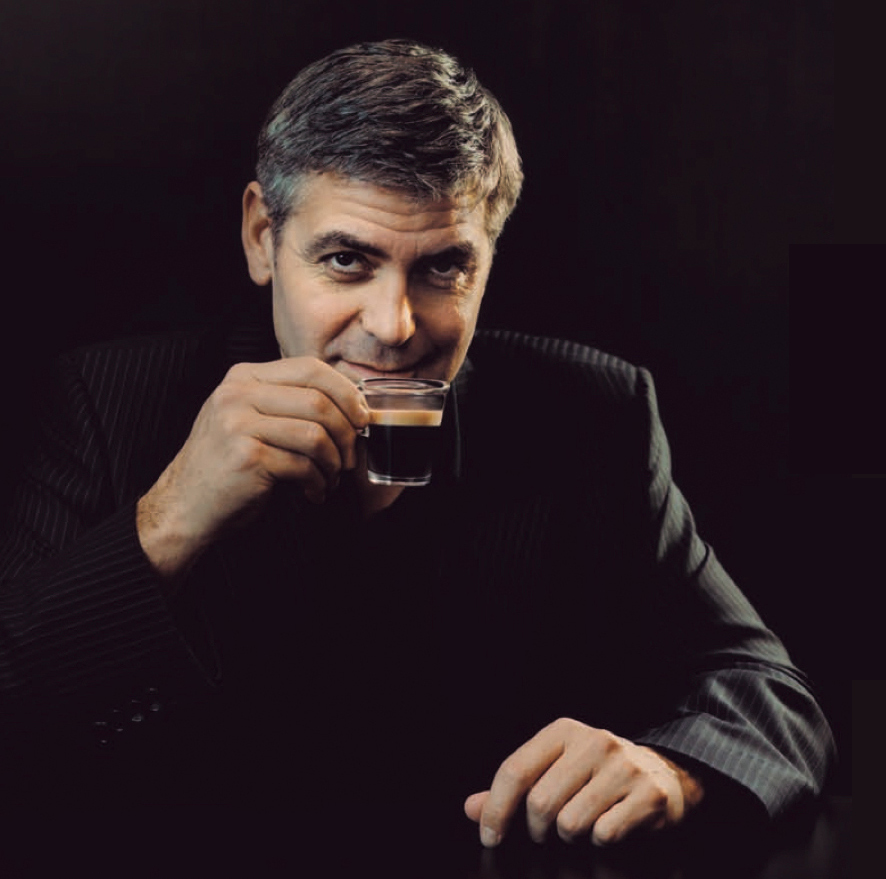
\includegraphics[height=7.5cm]{./pics/whatelse.jpg}

\end{frame}

\begin{frame}

    \frametitle{GLPI}

    \begin{block}{A nonprofit organisation}
        \begin{itemize}
            \item Indepnet, a French nonprofit association
            \item Since 2002
        \end{itemize}
    \end{block}

    \begin{block}{Two independant projects leaders}
        \begin{itemize}
            \item Jean-Mathieu Doléans
            \item Julien Dombre
        \end{itemize}
    \end{block}

    \begin{block}{Contributors and developers}
        \begin{itemize}
            \item 5 developers
            \item plugins developers
            \item translators
        \end{itemize}
    \end{block}

\end{frame}

\begin{frame}

    \frametitle{FusionInventory}

    \begin{block}{A sister project}
        \begin{itemize}
            \item Created by some people of the GLPI community
            \item Strong relationship with GLPI
        \end{itemize}
    \end{block}

    \begin{block}{A community}
        \begin{itemize}
            \item More than 10 people involved
            \item Supported by 2 companies
        \end{itemize}
    \end{block}

    \begin{block}{But also}
        \begin{itemize}
            \item Open minded : other projects are welcomed!
            \item Agent already used by third parties projects
        \end{itemize}
    \end{block}

\end{frame}

\section{Questions}

\begin{frame}
    \frametitle{Questions?}

%    \bf{Questions?}
    \begin{center}

    
\includegraphics[height=5cm]{./pics/question.pdf}

    \end{center}
%    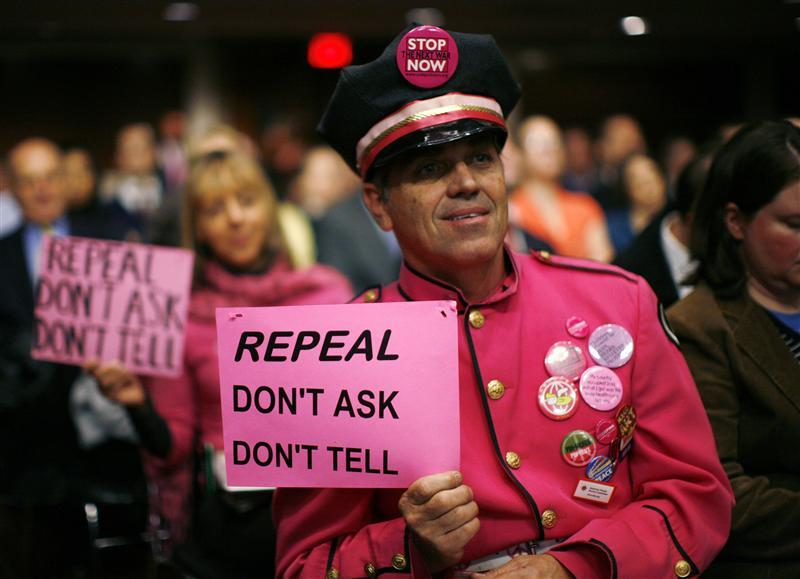
\includegraphics[height=7.5cm]{./pics/ask.jpg}

\end{frame}

\begin{frame}
    \frametitle{Thanks}

        \begin{itemize}
                \item Purchasing: \url{http://www.flickr.com/photos/epsos/5394616925/}
                \item LDAP: \url{http://www.flickr.com/photos/heyrocker/2954514315/}
                \item SSO: \url{http://www.flickr.com/photos/13519089@N03/1380483002/}
                \item User picture: \url{http://www.flickr.com/photos/wonderlane/5043174502/}
                \item Manager: \url{http://www.flickr.com/photos/eastcapital/5228405457/}
                \item Server: \url{http://www.flickr.com/photos/sylvar/31436963/}
                \item Helpdesk: \url{http://www.flickr.com/photos/runlevel0/2196587153/}
                \item Database: \url{http://www.flickr.com/photos/garryknight/5476230085/}
                \item Information: \url{http://www.flickr.com/photos/garryknight/5476230085/}
                \item Networking: \url{http://www.flickr.com/photos/dbreg2007/4376127852/}
                \item Printer: \url{http://www.flickr.com/photos/photofarmer/467241015/}
                \item House of cards: \url{http://www.flickr.com/photos/gibbons/2294375187/in/photostream/}
        \end{itemize}

\end{frame}



\end{document}
